\section{Interference}
\label{sec:interference}
We also conducted measurements outdoor near an interference source transmitting on the same frequency band as GPS. As we can see from the figure \ref{fig:interference_figure_3} the signal to noise ratio has a mean value of 23.9 dB.Hz which are values comparable with the ones obtained during the indoor measurement. While if we analyze the figure \ref{fig:interference_figure_4} we notice that the 50\% distribution of the measurements are inside a radius of 27.3 meters. The interference from external sources negatively affects the accuracy of the position estimate due to errors in the measured pseudoranges. This interference can occur because satellite signals are relatively weak, making them susceptible to degradation by other signals, such as those generated by television repeaters or other sources.
Interferences can be detected and be mitigated at receiver level through the use of antenna shaping, frequency filtering, time domain blanking, etc.
%What can we do to fighting against the interference problem? We need to deal with both detection and countermeasures.
%Since the interference affects the receiver at different levels in the same way we can act at different stages.
%We can observe different values throughout the processing chain, up to the pseudo range measurements and usually, the sooner you get it, the better is. 
%One thing we can monitor is the signal to noise ratio because since this is estimated by the receiver and the receiver cannot distinguish between noise and interference this ones are estimated like noise.
%The effect is that the signal to noise ratio is effected by the interference and we can set a threshold if the signal to noise ratio is below some threshold that means that might be an interference.


\begin{figure}[H]
  \begin{subfigure}{.22\textwidth}
  \centering
    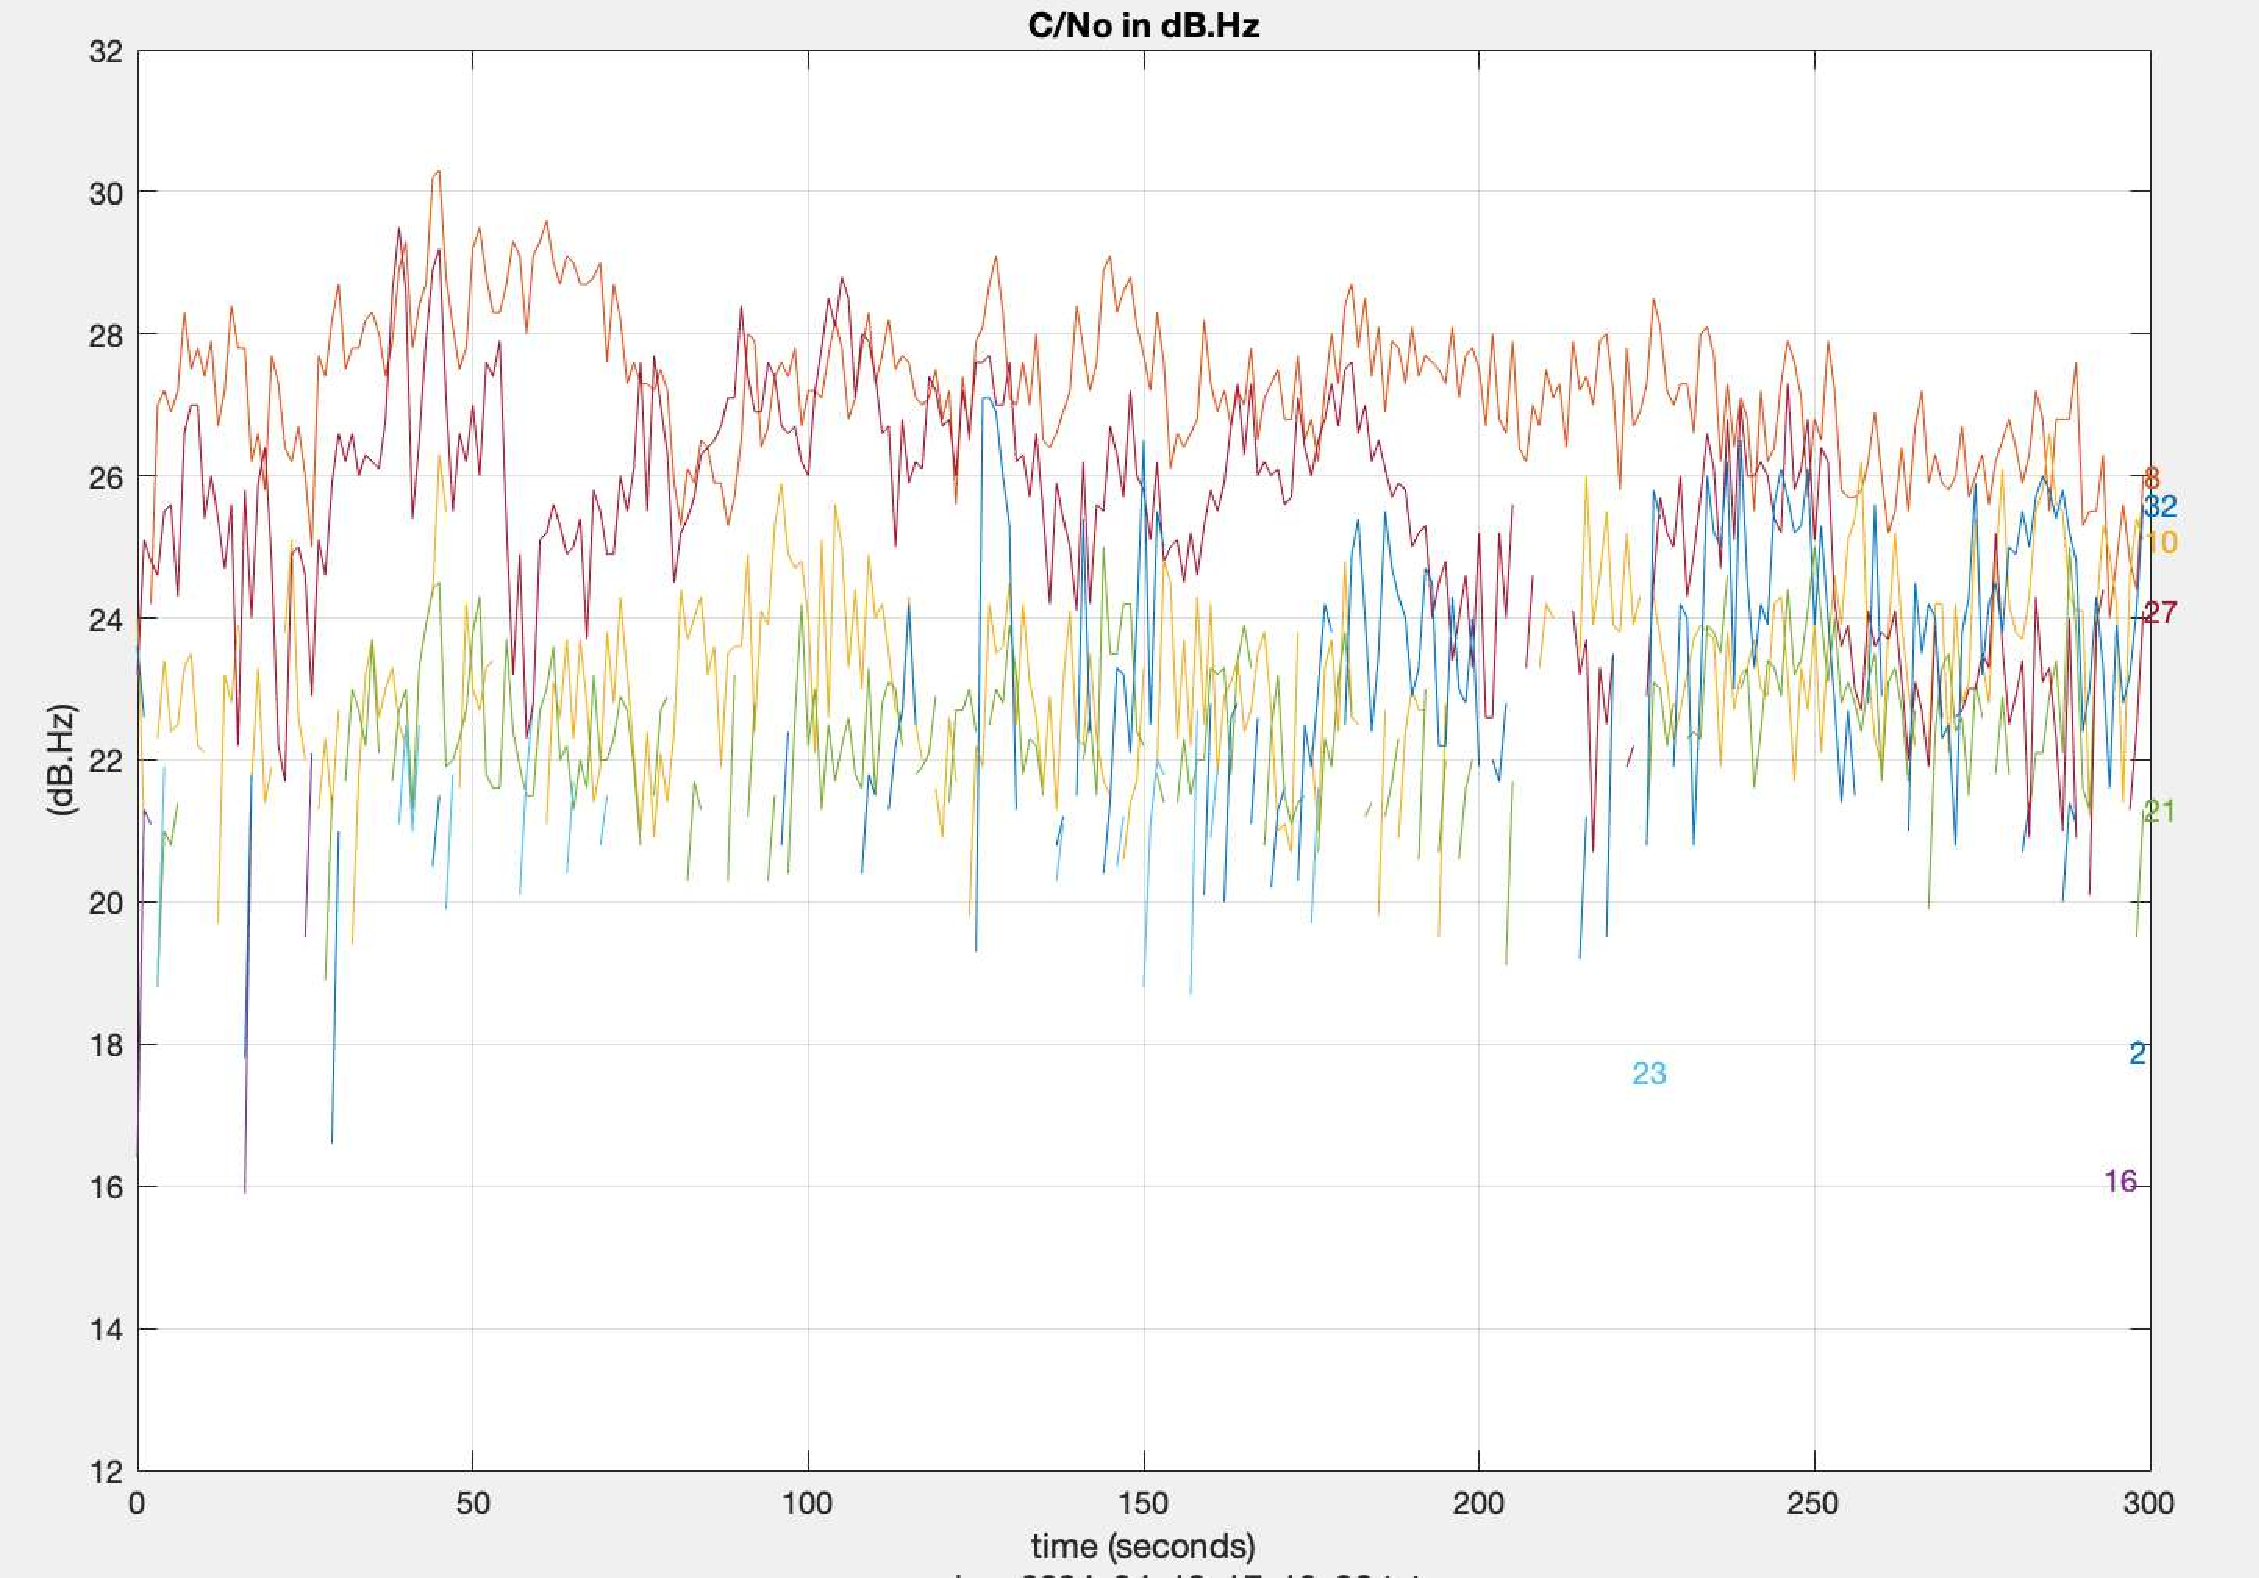
\includegraphics[width=1\linewidth]{images/interference_figure_3.pdf}
    \caption{C/N0 in dB.Hz}
    \label{fig:interference_figure_3}
  \end{subfigure}
  \begin{subfigure}{.22\textwidth}
  \centering
    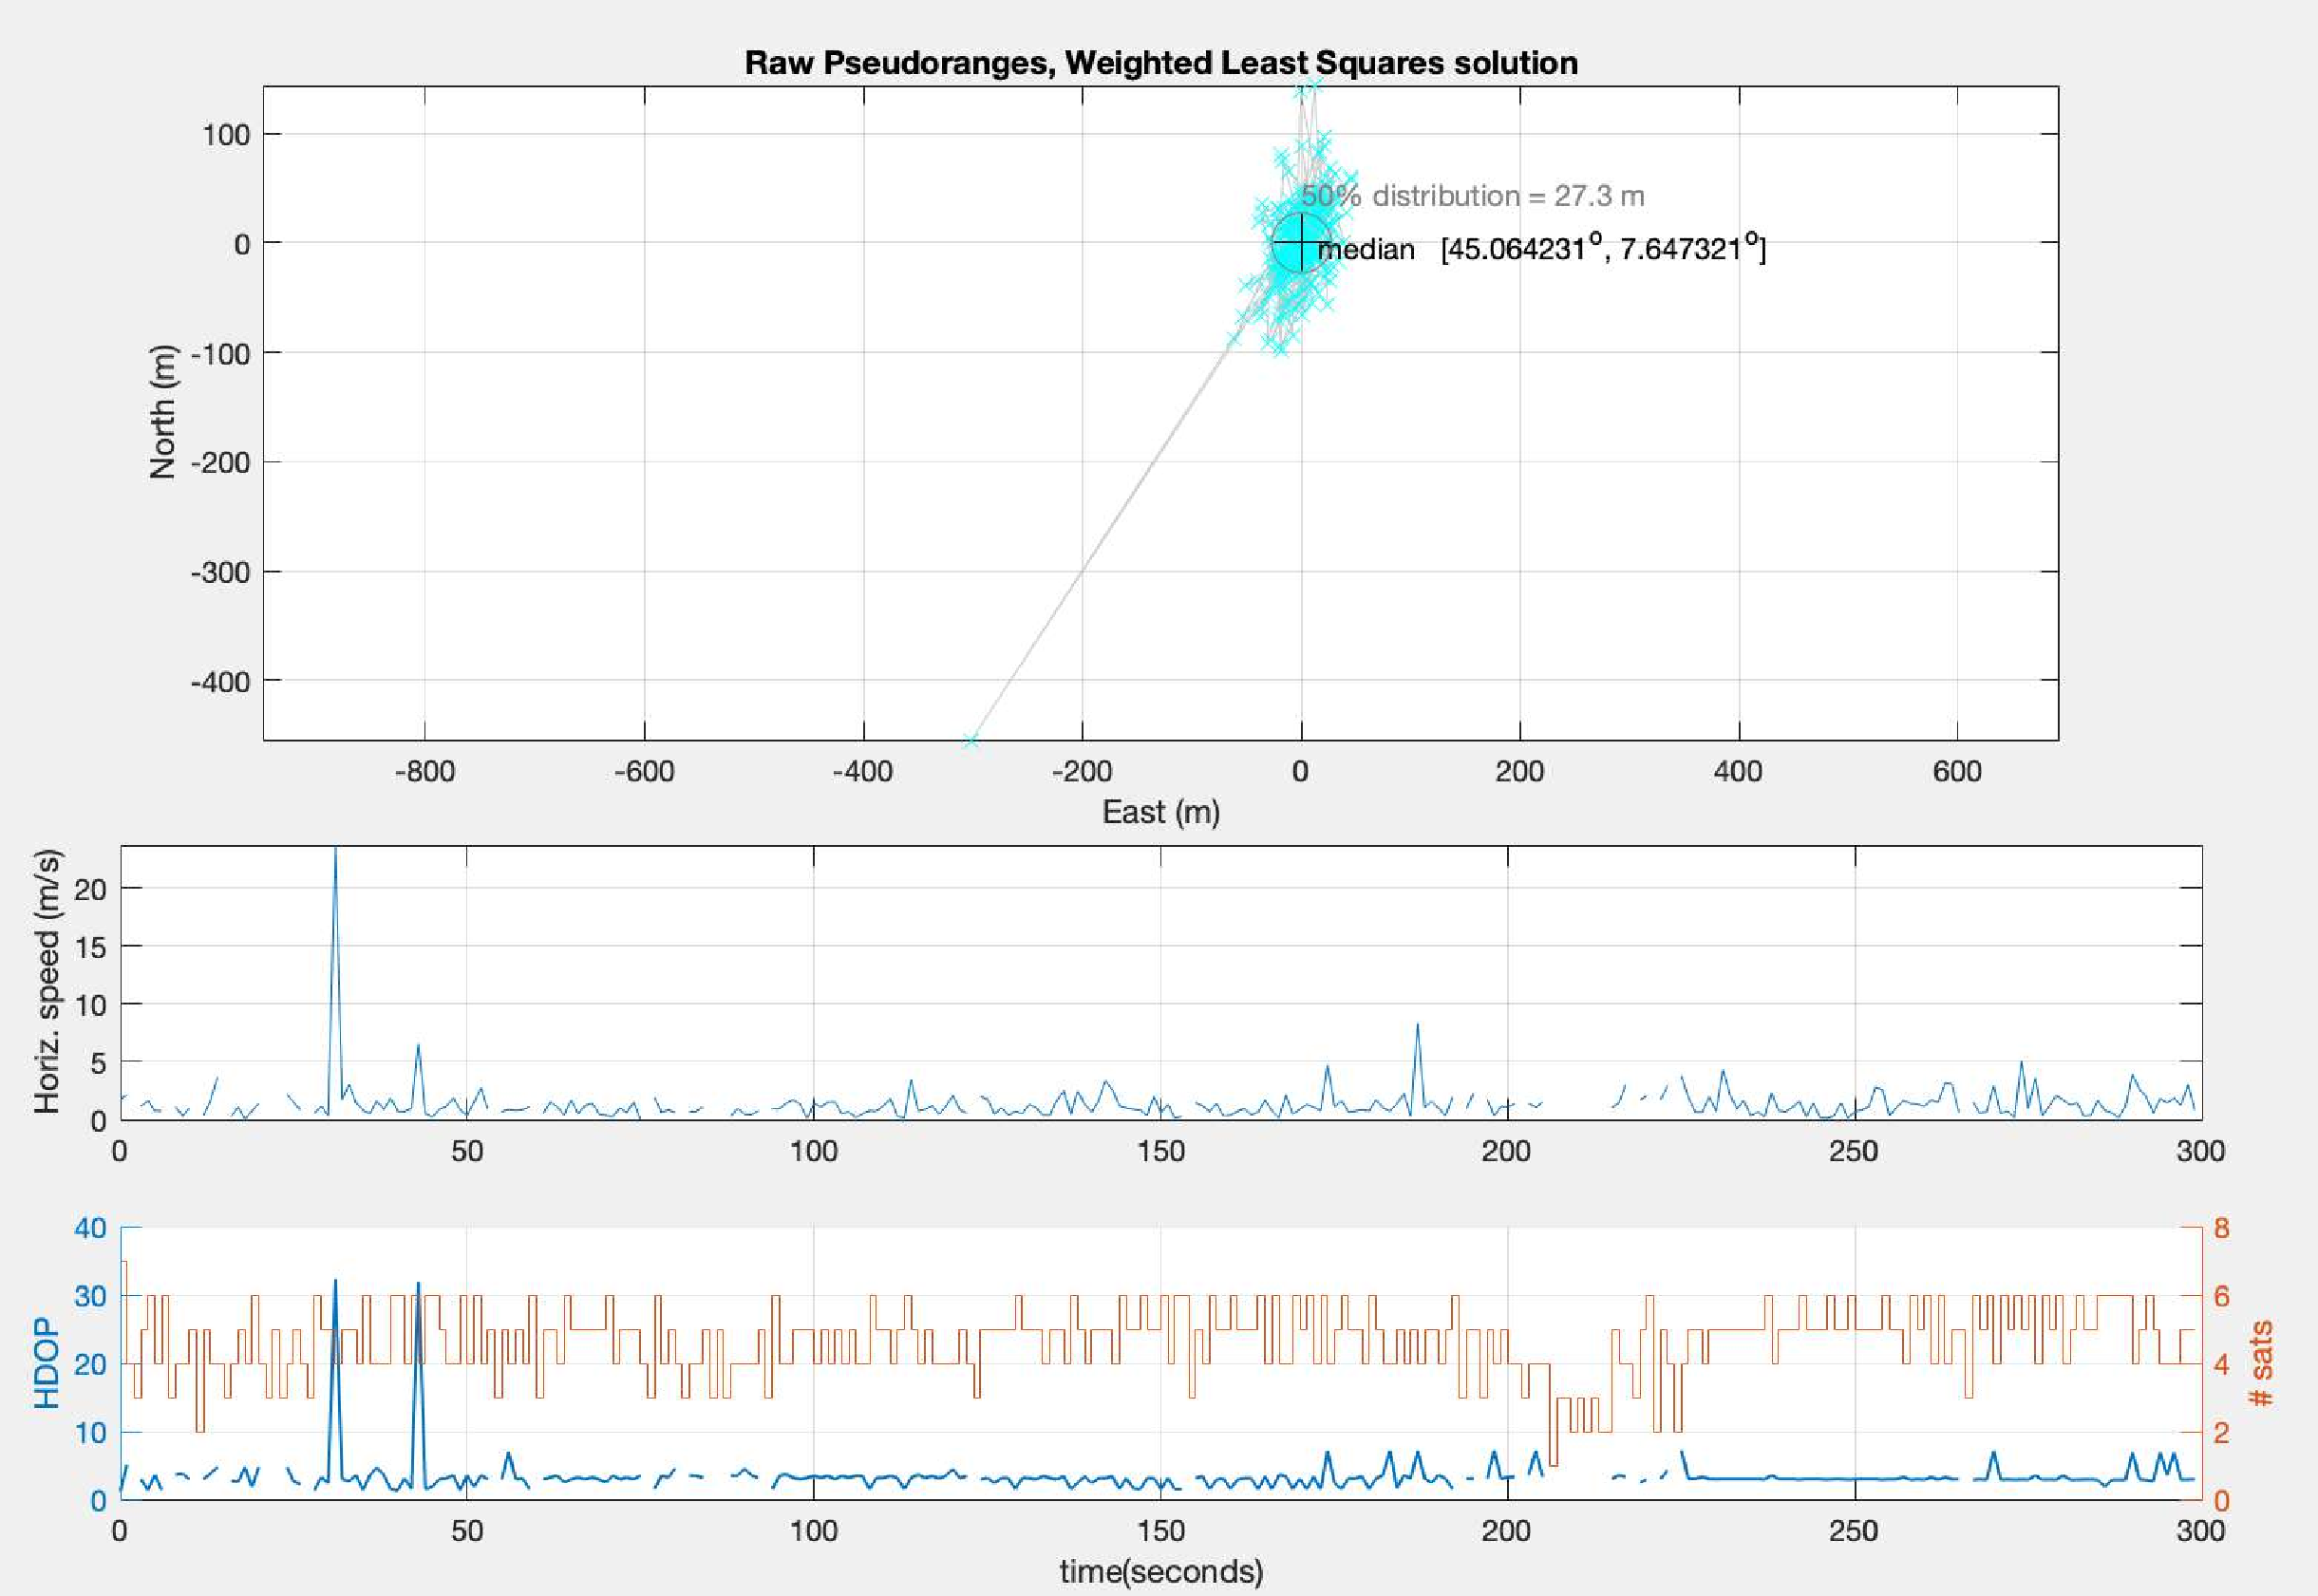
\includegraphics[width=1\linewidth]{images/interference_figure_4.pdf}
    \caption{Position estimate, Horizontal speed, HDOP}
    \label{fig:interference_figure_4}
  \end{subfigure}
  \vspace{10pt}
  %\caption{Positioning solution on map}
  %\captionsetup[subfigure]{position=below}
\end{figure}
